% L'outil Pint

\begin{frame}
  \frametitle{The Pint Tool}
  \framesubtitle{\tcite{\url{http://processhitting.wordpress.com}}}

\only<1>{

\begin{block}{Features}
   \begin{itemize}
      \item Free software (API available for future developments)
\item \textbf{Textual language} to describe a Process Hitting (GUI currently under development) 
%\begin{tabular}{ll}
\item \textbf{Implemented tools}:
  %&
   \begin{itemize}
      \item Translations from and to various other models
      \item Fixed points research
      \item Stochastic simulation
      \item Reachability checker
    \end{itemize}
%\end{tabular}
\end{itemize}
\end{block}

}

%\only<2>{
%\medskip
%\tval{Results and performance} (reachability analysis):
%
%\scalebox{0.9}{
%\begin{tabular}{|r||c|c|c|c||c|c|c|}
%\hline
%Model & sorts & procs & actions & states & Biocham\tscite{$^1$} & libddd\tscite{$^2$} & \Pint \\\hline
%egfr20 & 35 & 196 & 670 & $2^{64}$ & [3s-KO] & [1s-150s] & \tval{0.007s} \\\hline
%tcrsig40 & 54 & 156 & 301 & $2^{73}$ & [1s-KO] & [0.6s-KO] & \tval{0.004s} \\\hline
%tcrsig94 & 133 & 448 & 1124 & $2^{194}$ & KO & KO & \tval{0.030s} \\\hline
%egfr104 & 193 & 748 &  2356 & $2^{320}$ &  KO & KO & \tval{0.050s} \\\hline
%\end{tabular}
%}
%
%\footnotesize
%\tscite{$^1$} \tcite{Inria Paris-Rocquencourt/Contraintes}
%
%\footnotesize
%\tscite{$^2$} \tcite{LIP6/Move}
%}

\end{frame}

\begin{frame}
  \frametitle{The Mobyle portal}
  \framesubtitle{\tcite{\url{http://mobyle.biotempo.univ-nantes.fr/cgi-bin/portal.py}}}

\begin{block}{Presentation}
   \begin{itemize}
      \item \textbf{Web application unifying} tools for systems biology analysis
      \item Powered by the Mobyle framework 
      \item Project led by Julien \textsc{Gras} (French ANR \og BIOTempo \fg) 
    \end{itemize}
\end{block}

\only<1>{
\begin{figure}
  \begin{center}
  \scalebox{0.35}{
    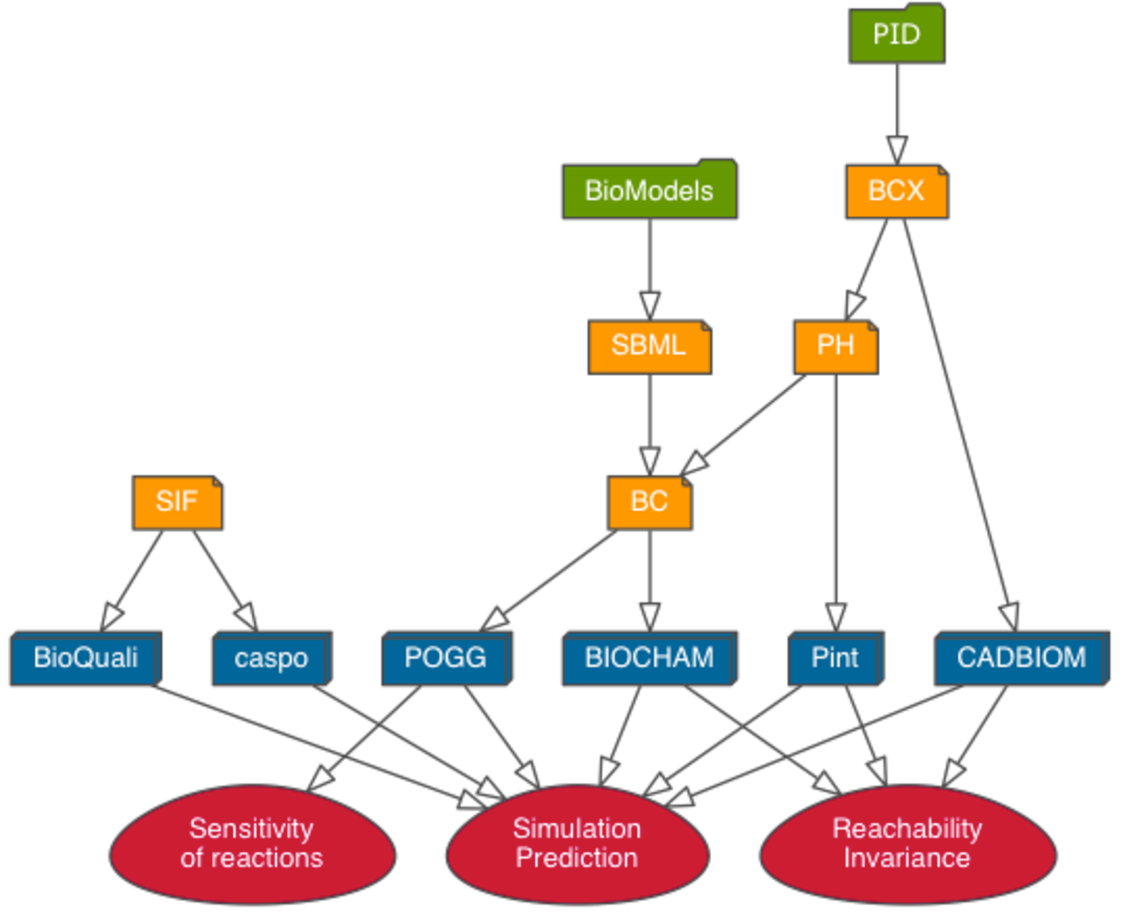
\includegraphics[width=\textwidth]{figures/biotempo-schema_global.pdf}
  }
    \caption{\label{fig:mobile} General architecture of the BIOtempo Mobyle server}
  \end{center}
\end{figure}
}

\only<2>{
\begin{figure}
  \begin{center}
  \scalebox{0.4}{
    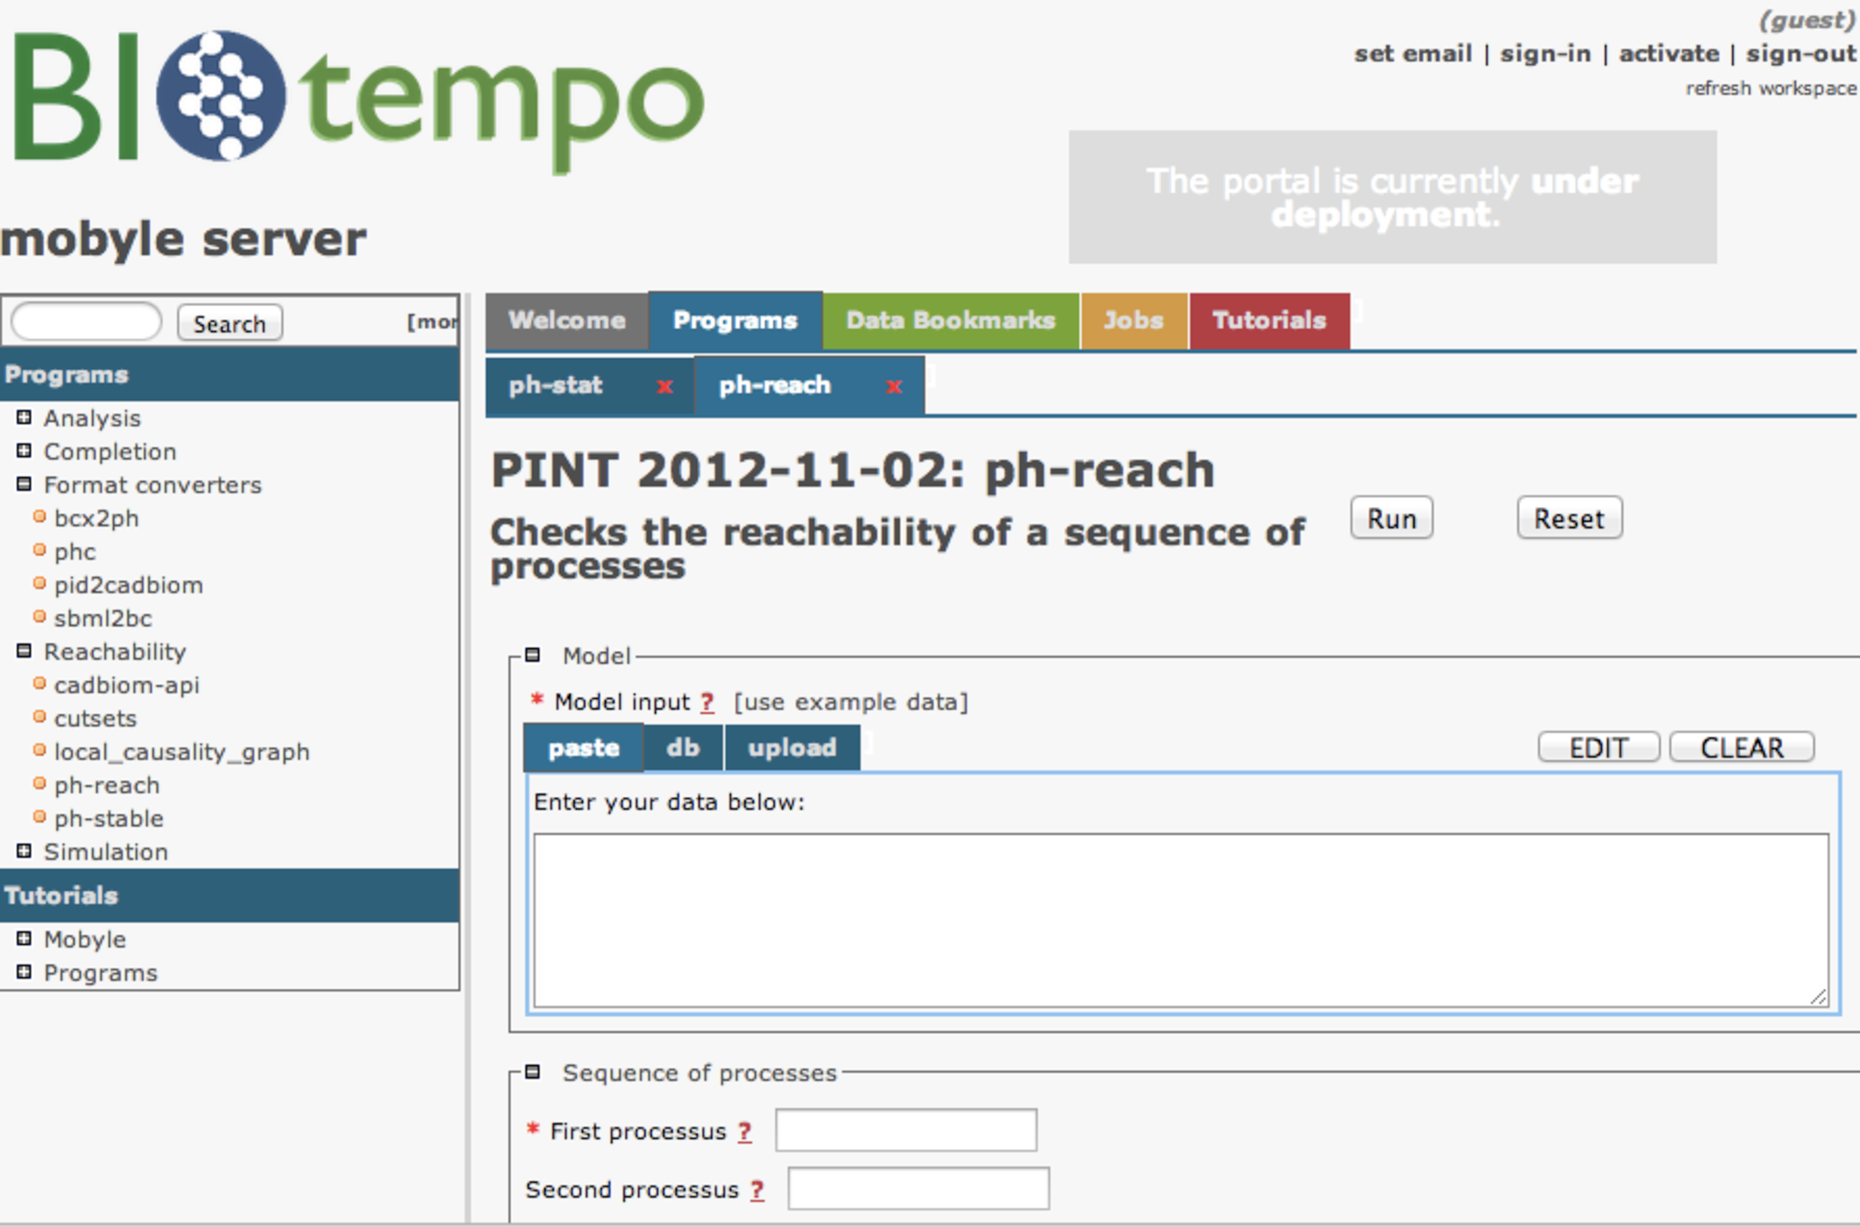
\includegraphics[width=\textwidth]{figures/biotempo-screenshot.pdf}
  }
    \caption{\label{fig:mobile} Screenshot from the BIOtempo Mobyle server: \url{http://mobyle.biotempo.univ-nantes.fr/cgi-bin/portal.py}}
  \end{center}
\end{figure}
}

\end{frame}
